\documentclass[11pt]{article}	
\pagestyle{plain}
\usepackage[english]{babel}
\usepackage{textcomp}
\usepackage[margin=1in]{geometry}
\usepackage{setspace}
\usepackage{booktabs}
\usepackage{tabularx}
\usepackage{graphicx}

\onehalfspacing

\begin{document}

\title{Trash Attack: Game Design Document}
\author{Selina Wang}
\date{}

\maketitle


Trash Attack is a fast-paced game that tests your reflexes. Defend against the incoming trash by sorting them into the right bins as they fall. Learn to remember how to sort your trash in a fun and easy way! How long can you last before the trash overwhelms you? The sustainability of the world's resources depends on you. 

\vspace{3 mm}

\textbf{Target Audience}: I aim to reach out to everyone! Lack of recycling is a widespread issue and I hope to teach as many people as possible about the proper way to recycle with this game. 

\vspace{3 mm}

\textbf{Platform}: iOS

\vspace{3 mm}


\textbf{Genre}: Arcade/Edutainment
\vspace{3 mm}


\textbf{Core Gameplay}: The player's role is to sort various items of trash as they fall from the sky by dragging them to the matching bin. The goal of the game is to collect as much trash in the right bins as possible before the player runs out of lives. As the game progresses, the trash falls faster and faster, making it harder not to miss an item. There are four bins: Metal, Glass \& Plastic; Paper \& Cardboard; Trash; and Other. 

\vspace{3 mm}

\textbf{Visual Style}: Trash Attack is a 2-D game. Its graphics are mostly cartoonish. 


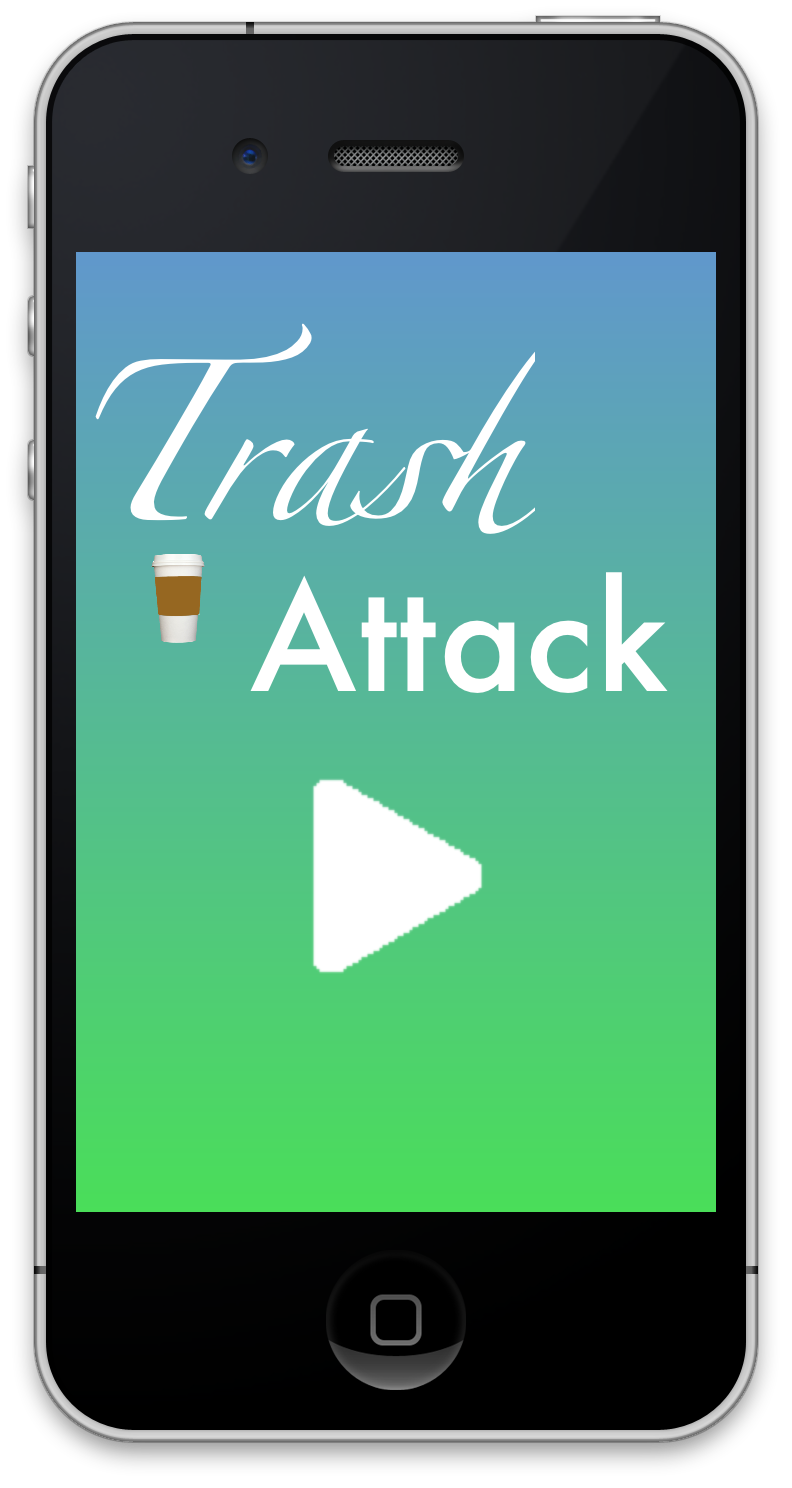
\includegraphics[scale=0.3]{loadingscreen}
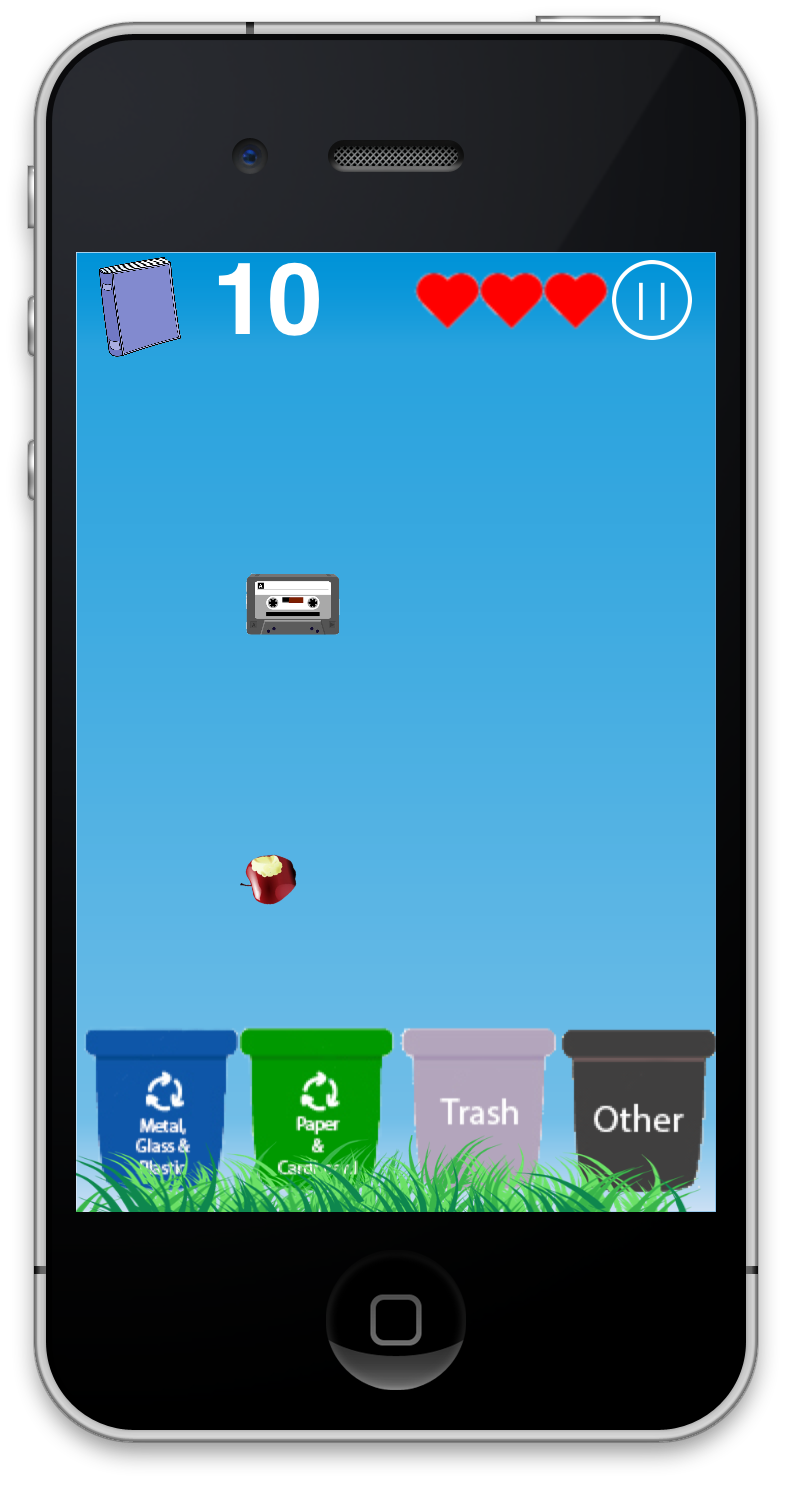
\includegraphics[scale=0.3]{gameplay1}
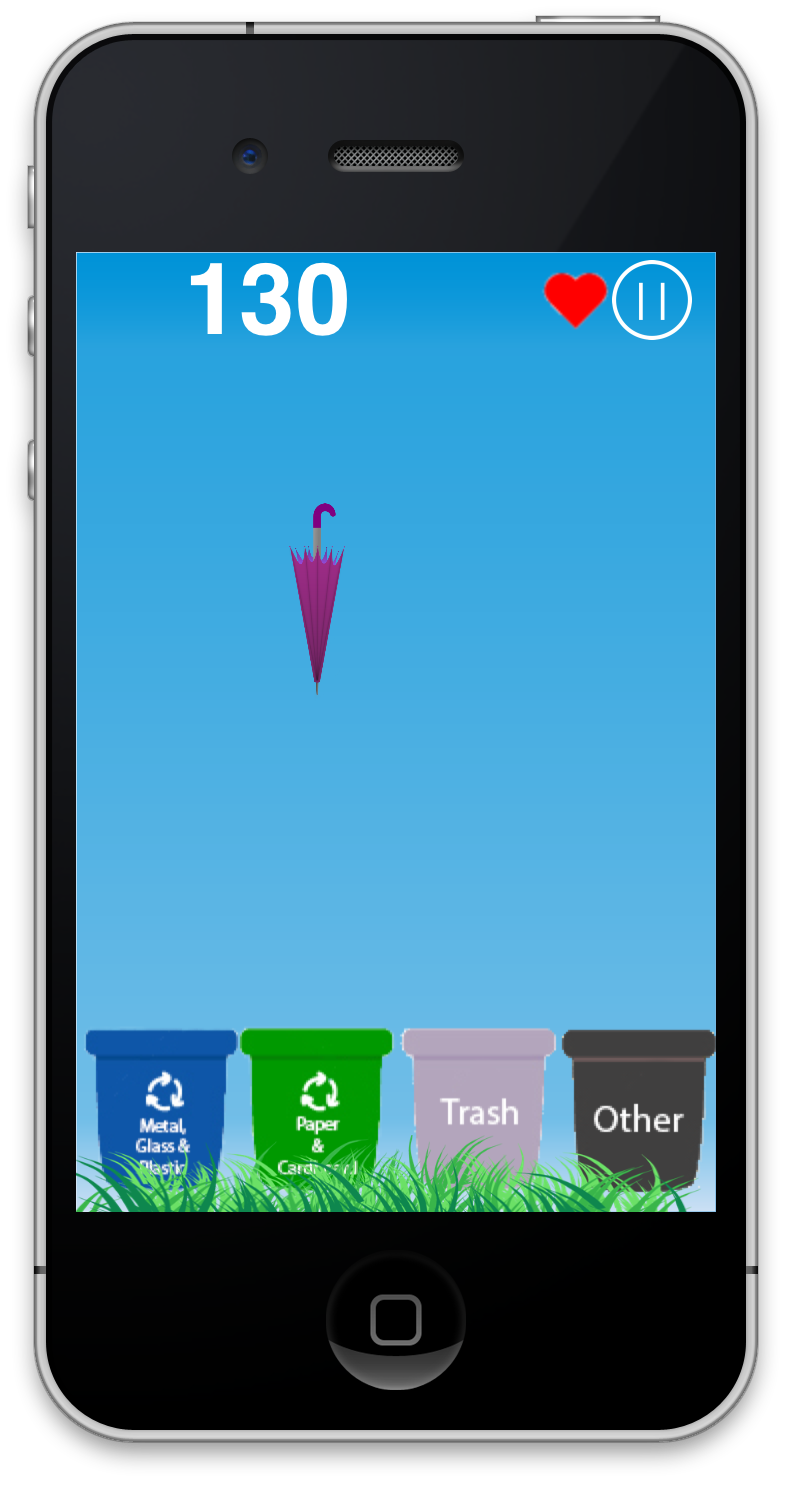
\includegraphics[scale=0.3]{gameplay2}



\newpage
\textbf{Future Improvements}: Currently, Trash Attack is in an early stage. It is a simple, engaging prototype that challenges users to sort trash as quickly as possible, thus training them to remember what items go in which bins. However, I haven't yet incorporated tutorials and information within the game that tells the user how to categorize each item. In addition, more visual feedback, such as a flash when the player categorizes an item correctly or incorrectly, or a popup when the user has a certain streak, would improve the user experience. I plan on adding levels in the future--introducing new, more difficult items as the player advances. 
\\[3ex]
Another possibility is to introduce different mechanics to keep the game interesting. Examples of such modes are multiple-choice questions, or, for instance, a mode where you tap as many items that match a certain bin in a certain amount of time.  Recycling can be complex; there are many different types of plastics, paper and metal, and an object can contain more than one type of material. There are also many ways to reuse objects creatively. This opens up all different kinds of modes. I could program a level where the player has to take apart a car, and recycle the parts individually, or a level that focuses specifically on the different ways an item can be reused. 
\\[3ex]
Less than half of the world's recyclable materials are recycled every day. It is imperative that people learn about how to recycle; thus, improving and expanding upon this game is of the utmost importance. 


\end{document}